\documentclass{article}
\usepackage{ctex}
\usepackage{amsmath}
\usepackage{amssymb}
\usepackage{amsthm}
\usepackage{graphicx}
\usepackage{hyperref}
\usepackage{geometry}
\usepackage{caption}
\usepackage{listings}
\usepackage{color}
\usepackage{tikz}
\usepackage{tikz-feynman}
\usepackage{slashed}


\newcommand{\Tr}{\mathbf{Tr}}


%%标题设置
\title{$e^{-} + e^{+} \to W^{-} + W^{+}$一阶树图散射截面计算}
\author{Kaiser}
\date{\today}



\begin{document}

%%设置标题与目录

\maketitle

\begin{center}
\tableofcontents
\end{center}
\newpage


%%导言区
\begin{abstract}
这篇文章主要是一次费曼图的计算练习,从而熟悉费曼图的计算方法。
计算过程:$e^{-} + e^{+} \to W^{+} + W^{-}$
计算的是树图,因此一共只有三个过程:

\begin{center}
    \begin{minipage}{0.32\textwidth}
        \centering
        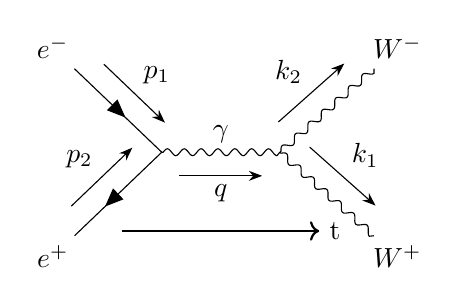
\begin{tikzpicture}[scale=0.5]
            \begin{feynman}
                \vertex (b);
                \vertex [above left=1.5cm of b] (a) {\(e^{-}\)};
                \vertex [below left=1.5cm of b] (e) {\(e^{+}\)};
                \vertex [right=1.5cm of b] (f); 
                \vertex [above right=1.5cm of f] (c) {\(W^{-}\)};
                \vertex [below right=1.5cm of f] (d) {\(W^{+}\)};
                
                \diagram* {
                    (a) -- [fermion,momentum={\(p_1\)}] (b),
                    (e) -- [anti fermion,momentum={\(p_2\)}] (b),
                    (b) -- [boson,momentum'={\(q\)},edge label={\(\gamma\)}] (f),
                    (f) -- [boson,momentum={\(k_1\)}] (d),
                    (f) -- [boson,momentum={\(k_2\)}] (c)
                };
            \end{feynman}
            \draw[->, thick] (-1,-2) -- (4,-2) node[right] {t};
        \end{tikzpicture}
    \end{minipage}
    \hfill
    \begin{minipage}{0.32\textwidth}
        \centering
        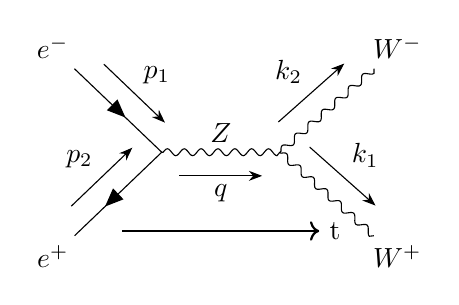
\begin{tikzpicture}[scale=0.5]
            \begin{feynman}
                \vertex (b);
                \vertex [above left=1.5cm of b] (a) {\(e^{-}\)};
                \vertex [below left=1.5cm of b] (e) {\(e^{+}\)};
                \vertex [right=1.5cm of b] (f); 
                \vertex [above right=1.5cm of f] (c) {\(W^{-}\)};
                \vertex [below right=1.5cm of f] (d) {\(W^{+}\)};
                
                \diagram* {
                    (a) -- [fermion,momentum={\(p_1\)}] (b),
                    (e) -- [anti fermion,momentum={\(p_2\)}] (b),
                    (b) -- [boson,momentum'={\(q\)},edge label={\(Z\)}] (f),
                    (f) -- [boson,momentum={\(k_1\)}] (d),
                    (f) -- [boson,momentum={\(k_2\)}] (c)
                };
            \end{feynman}
            \draw[->, thick] (-1,-2) -- (4,-2) node[right] {t};
        \end{tikzpicture}
    \end{minipage}
    \hfill
    \begin{minipage}{0.32\textwidth}
        \centering
        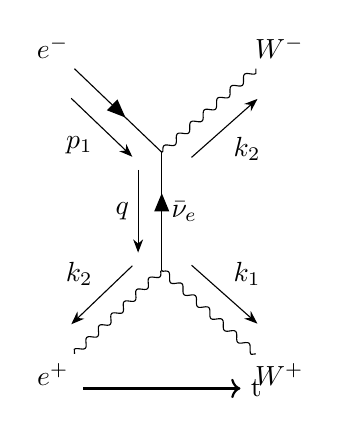
\begin{tikzpicture}[scale=0.5]
            \begin{feynman}
                \vertex (b);
                \vertex [above left=1.5cm of b] (a) {\(e^{-}\)};
                \vertex [above right=1.5cm of b] (c) {\(W^{-}\)};
                \vertex [below=1.5cm of b] (f); 
                \vertex [below left=1.5cm of f] (e) {\(e^{+}\)};
                \vertex [below right=1.5cm of f] (d) {\(W^{+}\)};
                
                \diagram* {
                    (a) -- [fermion,momentum'={\(p_1\)}] (b),
                    (b) -- [boson,momentum'={\(k_2\)}] (c),
                    (b) -- [anti fermion,momentum'={\(q\)},edge label={\(\bar{\nu}_e\)}] (f),
                    (f) -- [boson,momentum={\(k_1\)}] (d),
                    (f) -- [boson,momentum'={\(k_2\)}] (e)
                };
            \end{feynman}
            \draw[->, thick] (-2,-6) -- (2,-6) node[right] {t};
        \end{tikzpicture}
    \end{minipage}
\end{center}

接下来我们将先依次计算他们的散射振幅 $M_{\gamma},M_{Z},M_{\bar{\nu}_e}$,然后再计算出总散射截面,最终可视化各个过程的散射截面对总散射截面的贡献。
\end{abstract}


%%正文区




\section{从拉格朗日量到费曼规则}

\subsection{QED 的费曼规则}
首先,我们给出带协变规范固定项的 QED 拉格朗日量\cite{weinzierl2025feynmandiagrams}:
\begin{equation}
    \mathcal{L}_{QED} = \frac{1}{2}A^{\mu}(x) \left[\Box g_{\mu\nu} + \left(1 - \frac{1}{\xi} \partial_{\mu}\partial^{\nu}\right)\right]A^{\nu}(x) + \bar{\psi}(x)\left(i\gamma^{\mu}\partial_{\mu} - m\right)\psi(x) - e\bar{\psi}(x)\gamma^{\mu}A_{\mu}(x)\psi(x)
\end{equation}

其中,$A^{\mu}(x)$ 是光子场,$\psi(x)$ 是电子场, $\Box$ 为达朗贝尔算符,$g_{\mu\nu}$ 是闵可夫斯基度规,$\xi$ 是规范固定参数,$m$ 是电子质量,$e$ 是电子电荷。

接下来,我们将拉格朗日量转化为费曼规则,首先考虑第一部分:
\begin{equation}
    \mathcal{L}_{A} = \frac{1}{2}A^{\mu}(x) \left[\Box g_{\mu\nu} + \left(1 - \frac{1}{\xi} \partial_{\mu}\partial^{\nu}\right)\right]A^{\nu}(x)
\end{equation}

首先简写一下,将中间部分定义为一个大的算符 $P_{\mu\nu}(x)$,
\begin{equation}
    P_{\mu\nu}(x) = \Box g_{\mu\nu} + \left(1 - \frac{1}{\xi} \partial_{\mu}\partial^{\nu}\right)
\end{equation}

接着将我们的拉格朗日量通过傅里叶变换进入到动量空间当中,
\begin{equation}
    A_{\mu}(x) = \int \frac{d^{D}q}{\left(2\pi\right)^D} e^{-iq\cdot x}\tilde{A}_{\mu}(q)
\end{equation}

于是我们有:
\begin{equation}
    \partial_{\mu} \to -iq_{\mu},\qquad\qquad \Box \to -q^2
\end{equation}

通过这个变换,我们将可以把 $P_{\mu\nu}(x)$ 写成:
\begin{equation}
    P_{\mu\nu}(q) = -q^2 g_{\mu\nu} + \left(1 - \frac{1}{\xi}\right)q_{\mu}q_{\nu}
\end{equation}

考虑到,$P_{\mu\sigma}(q)\left(P^{-1}\right)^{\sigma\nu}(q)$ 求得为 $g_\mu^\nu = I$,因此我们设逆矩阵的形式为
\begin{equation}
    (P^{-1})^{\mu\nu} = a(q)g_{\mu\nu} + b(q)\frac{q_{\mu}q_{\nu}}{q^2}
\end{equation}

代入进行计算,便可以求得 $a(q),b(q)$
\begin{equation}
    a(q) = -\frac{1}{q^2},\qquad b(q) = \frac{1 - \xi}{q^2}
\end{equation}

因此我们可以得到
\begin{eqnarray}
    (P^{-1})^{\mu\nu} &=& -\frac{1}{q^2}g^{\mu\nu} + \frac{1 - \xi}{q^4}q^{\mu}q^{\nu} \\
    &=& \frac{i}{q^2}\left[ig^{\mu\nu} - i\left(1 - \xi\right)\frac{q^{\mu}q^{\nu}}{q^2}\right]
\end{eqnarray}

接下来,再乘上一个 $i$,我们就可以得到光子传播子的费曼规则:
\begin{equation}
    G^{\mu\nu} = \frac{i}{q^2}\left[-g^{\mu\nu} + \left(1 - \xi\right)\frac{q^{\mu}q^{\nu}}{q^2}\right]
\end{equation}

其费曼图我们表示为
\begin{center}
    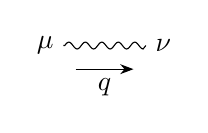
\begin{tikzpicture}[scale=0.5]
        \begin{feynman}
            \vertex (a) {\(\mu\)};
            \vertex [right=1.5cm of a] (b) {\(\nu\)};

            \diagram* {
                (a) -- [boson,momentum'={\(q\)}] (b)
            };
        \end{feynman}
    \end{tikzpicture}
\end{center}

接着我们考虑第二部分:
\begin{equation}
    \mathcal{L}_{ee} = \bar{\psi}(x)\left(i\gamma^{\mu}\partial_{\mu} - m\right)\psi(x)
\end{equation}
首先我们将拉格朗日量进行傅里叶变换,得到:
\begin{equation}
    \mathcal{L}_{ee} = \bar{\tilde{\psi}}(q)\left(\slashed{q} - m\right)\tilde{\psi}(q)
\end{equation}

和在计算光子传播子过程一样,我们让
\begin{equation}
    \left(\slashed{q} - m\right)S_F(q) = 1
\end{equation}

求解并乘上 $i$ 可得费曼传播子
\begin{equation}
    S_F(q) = \frac{i}{\slashed{q} - m} = \frac{i(\slashed{q} + m)}{q^2 - m^2}
\end{equation}

而我们的第三项,是一个光子场和两个电子场的耦合项,通过这一项,我们可以得到电子光子相互作用的顶点因子,还是给出这一部分的拉格朗日量
\begin{equation}
    \mathcal{L}_{e\gamma} = e\bar{\psi}(x)\gamma^{\mu}A_{\mu}(x)\psi(x)
\end{equation}

同样的,我们将拉格朗日量进行傅里叶变换,得到:
\begin{equation}
    \mathcal{L}_{e\gamma e} = e\int \frac{d^D p^\prime}{(2\pi)^D} \frac{d^D q}{(2\pi)^D} \frac{d^D p}{(2\pi)^D} e^{i(p_2 + p_1 - q)x} \bar{\tilde{\psi}}(p_2)\gamma^{\mu}\tilde{A}_{\mu}(q)\tilde{\psi}(p_1)
\end{equation}

我们考虑的过程是一个 $e^{-} + e^{+} \to \gamma$ 的正负电子对湮灭过程,通过观察一下我们的指数部分,得到动量守恒的条件
\begin{equation*}
    p_2 + p_1 = q
\end{equation*}

接下来继续计算一下 $S Matrix$ 矩阵元,
\begin{equation}
    S = T \exp\left(\int d^D x \mathcal{L}_{e\gamma e}(x)\right)
\end{equation}

我们可以得到其一阶围绕展开部分
\begin{equation*}
    S^{1} = i \int d^D x \mathcal{L}_{e\gamma e}(x)
\end{equation*}

计算可以得到
\begin{equation*}
    S^{1} = i e\int \frac{d^D p^\prime}{(2\pi)^D} \frac{d^D q}{(2\pi)^D} \frac{d^D p}{(2\pi)^D} (2\pi)^{D} \delta^{D}(p_2 + p_1 - q) \bar{\tilde{\psi}}(p_2)\gamma^{\mu}\tilde{A}_{\mu}(q)\tilde{\psi}(p_1)
\end{equation*}

从中,我们可以得到一个部分,也就是我们的 $e^{-}\gamma e^{+}$ 顶点因子 
\begin{equation}
    \mathcal{V}_{\mu} = -ie\gamma^{\mu}
\end{equation}

其对应的费曼图为
\begin{center}
    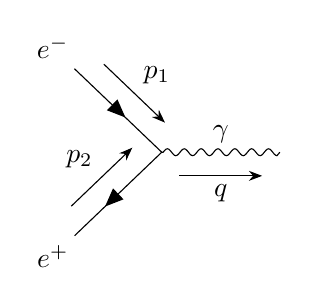
\begin{tikzpicture}[scale=0.5]
        \begin{feynman}
            \vertex (b);
            \vertex [above left=1.5cm of b] (a) {\(e^{-}\)};
            \vertex [below left=1.5cm of b] (e) {\(e^{+}\)};
            \vertex [right=1.5cm of b] (f);
            \diagram* {
                (a) -- [fermion,momentum={\(p_1\)}] (b),
                (e) -- [anti fermion,momentum={\(p_2\)}] (b),
                (b) -- [boson,momentum'={\(q\)},edge label={\(\gamma\)}] (f)
            };
        \end{feynman}
    \end{tikzpicture}
\end{center}

到此我们几乎计算完了我们的 $QED$ 当中的所有的顶点因子。








\subsection{电弱理论的费曼规则}

\subsubsection{从 $QED$ 的计算当中得到的一些启发}
在本节的前面一般的部分,我们示例性的计算出来了 $QED$ 的费曼规则,接下来我们需要计算的是 $SU(2)_{L} \times U(1)_{Y}$ 的费曼规则,但在计算前,我们先给一个比较基本的目标(这时我们从计算 $QED$ 的过程当中得到的一些经验)
\begin{table}[hbpt]
    \centering
    \begin{tabular}{ccc}
        \hline
        结构 & 来源 & 费曼规则 \\
        \hline
        二次项 & 规范场的动能项、质量项 & 传播子 \\
        \hline
        三次项、四次项(甚至更多) & 规范场的相互作用项 & 顶点因子 \\
        \hline
    \end{tabular}
\end{table}

\subsubsection{电弱理论的拉格朗日量}
接下来我们给出电弱理论的拉格朗日量,我们将其分成三项,分别是自由动能项、质量项和规范固定项\cite{commins1985weak}:
\begin{eqnarray}
    \mathcal{L}_{kinetic} &=& -\frac{1}{4}W_{\mu\nu}^{a}W^{a\mu\nu} - \frac{1}{4}B_{\mu\nu}B^{\mu\nu} \\
    \mathcal{L}_{mass} &=& m_W^2 W_{\mu}^+ W^{-\mu} + \frac{1}{2}m_Z^2 Z_{\mu}Z^{\mu} \\
    \mathcal{L}_{GF} &=& - \frac{1}{2\xi_W} \mathbf{Re}\left[\left(\partial^\mu W_\mu^{+}\right)\left(\partial^\nu W_{\nu}^{-}\right)\right] - \frac{1}{2\xi_Z} \left(\partial^\mu Z_\mu\right)\left(\partial^\nu Z_{\nu}\right) - \frac{1}{2\xi_{\gamma}} \left(\partial^\mu A_\mu\right)\left(\partial^\nu A_{\nu}\right)
\end{eqnarray}

其中,
\begin{enumerate}
    \item $\textcolor{blue}{W_{\mu\nu}^{a} = \partial_mu W_{\nu}^a - \partial_\nu W_{\mu}^a} + \textcolor{red}{g \epsilon_{\ bc}^{a}W_\mu^b W_\nu^c}$,此为 $SU(2)$的规范场强,蓝色的部分为 $W^+ W^-$ 的动能项,红色部分为非阿贝尔项,也导致了三规范玻色子耦合;
    \item $B_{\mu\nu} = \partial_\mu B_\nu - \partial_\nu B_\mu$,此为 $U(1)$的规范场强; 
\end{enumerate}

这两项便是所有的电弱玻色子的相互作用来源,这时候我们再引入玻色子(也就是我们在质量项和规范固定项当中所提到的)
\begin{eqnarray}
    W_\mu^{\pm} &=& \frac{1}{\sqrt{2}}(W_\mu^1 \mp i W_\mu^2) \label{eq1}\\
    Z_\mu &=& \cos\theta_W W_\mu^3 - \sin\theta_WB_\mu \label{eq2}\\
    A_\mu &=& \sin\theta_W W_\mu^3 + \cos\theta_W B_\mu \label{eq3}
\end{eqnarray}
电磁相互作用耦合常数(电荷)为: $e = g \sin\theta_W$



\subsubsection{拉格朗日量的展开}
接下来我们需要做的,将拉格朗日量当中的指标缩并给展开(这是真让人头大,算了我小半天终于展开完了,不难,但是小细节挺多的,一停下来就忘了自己刚刚算到哪儿了)。

第一步,我们将规范场 $W_\mu^1,W_\mu^2,W_\mu^3,B_\mu$ 给转化为规范玻色子的形式(即 $W_{\mu}^+,W_{\mu}^-,Z_\mu,A_{\mu}$),通过式 \eqref{eq1},\eqref{eq2},\eqref{eq3} 可以得到:
\begin{eqnarray}
    W_\mu^1 &=& \frac{1}{\sqrt{2}} \left(W_{\mu}^{-} + W_{\mu}^{+}\right) \label{eq4}\\
    W_\mu^2 &=& \frac{1}{i\sqrt{2}} \left(W_{\mu}^{-} - W_{\mu}^{+}\right) \label{eq5}\\
    W_\mu^3 &=& A_\mu \sin{\theta_W} + Z_\mu \cos{\theta_W} \label{eq6}\\
    B_\mu &=& A_\mu \cos{\theta_W} - Z_\mu \sin{\theta_W} \label{eq7}
\end{eqnarray}

这也就有
\begin{eqnarray}
    \partial_\mu W_\nu^1 -\partial_\nu W_\mu^1 &=& \frac{1}{\sqrt{2}} \left[\left(\partial_\mu W_\nu^- - \partial_\nu W_\mu^-\right) + \left(\partial_\mu W_\nu^+ - \partial_\nu W_\mu^+\right)\right] \label{eq8}\\
    \partial_\mu W_\nu^2 -\partial_\nu W_\mu^2 &=& \frac{1}{i\sqrt{2}} \left[\left(\partial_\mu W_\nu^- - \partial_\nu W_\mu^-\right) - \left(\partial_\mu W_\nu^+ - \partial_\nu W_\mu^+\right)\right] \label{eq9}
\end{eqnarray}

第二步,我们需要将我们刚刚得到的式 \eqref{eq8}、\eqref{eq9}、\eqref{eq6}、\eqref{eq7} 代入到拉格朗日量当中,得到

\begin{eqnarray}
    \mathcal{L}_{kinetic}^{W^{\pm}} &=& -\frac{1}{4}\left(\partial_\mu W_\nu^1 - \partial_\nu W_\mu^1\right)^2 -\frac{1}{4}\left(\partial_\mu W_\nu^2 - \partial_\nu W_\mu^2\right)^2 \nonumber\\
    &=& -\frac{1}{8} \left[\left(\partial_\mu W_\nu^- - \partial_\nu W_\mu^-\right) + \left(\partial_\mu W_\nu^+ - \partial_\nu W_\mu^+\right)\right] \left[\left(\partial^\mu W^{\nu-} - \partial^\nu W^{\mu-}\right) + \right. \nonumber\\
    && \left.\left(\partial^\mu W^{\nu+} - \partial^\nu W^{\mu+}\right)\right] +\frac{1}{8} \left[\left(\partial_\mu W_\nu^- - \partial_\nu W_\mu^-\right) - \right. \nonumber\\
    && \left.\left(\partial_\mu W_\nu^+ - \partial_\nu W_\mu^+\right)\right] \left[\left(\partial^\mu W^{\nu-} - \partial^\nu W^{\mu-}\right) - \left(\partial^\mu W^{\nu+} - \partial^\nu W^{\mu+}\right)\right] \nonumber\\
    &=& -\frac{1}{4}\left[\left(\partial_\mu W_\nu^- - \partial_\nu W_\mu^-\right)\left(\partial^\mu W^{\nu+} - \partial^\nu W^{\mu+}\right) + \left(\partial^\mu W^{\nu-} - \partial^\nu W^{\mu-}\right)\left(\partial_\mu W_\nu^+ - \partial_\nu W_\mu^+\right)\right] \nonumber \\
    &=& -\frac{1}{2} \left(\partial_\mu W_\nu^+ - \partial_\nu W_\mu^+\right)\left(\partial^\mu W^{\nu-} - \partial^\nu W^{\mu-}\right) \nonumber
\end{eqnarray}

接着再添加上我们的规范固定项和质量项,就可以得到 $W^{\pm}$ 玻色子的自由拉格朗日量
\begin{equation}
    \mathcal{L}_{free}^{W^{\pm}} = -\frac{1}{2} \left(\partial_\mu W_\nu^+ - \partial_\nu W_\mu^+\right)\left(\partial^\mu W^{\nu-} - \partial^\nu W^{\mu-}\right) + \frac{1}{2\xi_W} \mathbf{Re}\left[\left(\partial^\mu W_\mu^{+}\right)\left(\partial^\nu W_{\nu}^{-}\right)\right] + m_W^2 W_{\mu}^+ W^{-\mu}
\end{equation}

与计算 QED 时一样,我们将拉格朗日量转化到动量空间当中,主要的变换关系为
\begin{equation}
    \partial_\mu \to -ip_\mu,\qquad\qquad \partial^\mu \to -ip^\mu
\end{equation}

首先是将 $W^{\pm}$ 的场变换到动量空间当中
\begin{eqnarray*}
    W_\mu^+ &=& \int \frac{d^4p}{(2\pi)^4} e^{-ip\cdot x} \tilde{W}_\mu^+(p) \\
    W_\mu^- &=& \int \frac{d^4p}{(2\pi)^4} e^{-ip\cdot x} \tilde{W}_\mu^-(p) 
\end{eqnarray*}

接着便可得到动量空间的拉格朗日量
\begin{eqnarray*}
    \mathcal{L}_{kinetic}^{W^\pm}(p) &=& \frac{1}{2} \left(p_\mu p^\mu \tilde{W}_\nu^+ \tilde{W}^{-\nu} - p_\mu p^\nu \tilde{W}_\nu^+ \tilde{W}^{-\mu} - p_\nu p^\mu \tilde{W}_\mu^+ \tilde{W}^{-\nu} + p_\nu p^\nu \tilde{W}_\mu^+ \tilde{W}^{-\mu}\right) \\
    &=& p^2 g^{\mu\nu} \tilde{W}_\mu^+ \tilde{W}_{\nu}^{-} - \left(p \cdot \tilde{W}^+\right)\left(p \cdot \tilde{W}^-\right) \\
    \mathcal{L}_{mass}^{W^{\pm}} &=& m_W^2 \tilde{W}_\mu^+ \tilde{W}^{-\mu} = m_w^2 \tilde{W}_\mu^+ g^{\mu\nu} \tilde{W}_{\nu}^{-} \\
    &=& g^{\mu\nu} m_w^2 \tilde{W}_\mu^+ \tilde{W}_{\nu}^{-} \\
    \mathcal{L}_{gauge}^{W^{\pm}} &=& -\frac{1}{2\xi_W} 2\left(-ip_\mu\tilde{W}_\mu^+\right)\left(-ip^\nu \tilde{W}^{-\nu}\right)\\
    &=& \frac{1}{\xi_W} \left(p \cdot \tilde{W}^+\right)\left(p \cdot \tilde{W}^-\right) \\
    \mathcal{L}_{free}^{W^\pm} &=& \mathcal{L}_{kinetic}^{W^\pm} + \mathcal{L}_{mass}^{W^{\pm}} + \mathcal{L}_{gauge}^{W^{\pm}} \\
    &=& -\tilde{W}_\mu^+ \left[-\left(p^2 - m_W^2\right)g^{\mu\nu} + \left(1 - \frac{1}{\xi_W}\right)p^\mu p^\nu\right] \tilde{W}_{\nu}^{-}
\end{eqnarray*}

和之前在计算 $QED$ 的时候一样,我们可以得到 $W^{\pm}$ 的传播子
\begin{equation}
    D_{\mu\nu}^{W^\pm}(p) = -\frac{i}{p^2 - m_W^2}\left[g_{\mu\nu} + \frac{p_\mu p_\nu}{p^2 - m_W^2 \xi}\left(\xi_W - 1\right)\right]
\end{equation}



同理,我们还可以计算得出 $Z$ 玻色子的传播子以及电弱理论的光子的自由拉格朗日量为
\begin{eqnarray}
    \mathcal{L}_{free}^{Z}(p) &=& -\tilde{Z}_\mu^+ \left[-\left(p^2 - m_Z^2\right)g^{\mu\nu} + \left(1 - \frac{1}{\xi_Z}\right)p^\mu p^\nu\right] \tilde{Z}_{\nu}^{-} \\
    \mathcal{L}_{free}^{\gamma}(p) &=& -\tilde{A}_\mu^+ \left[-p^2 g^{\mu\nu} + \left(1 - \frac{1}{\xi_\gamma}\right)p^\mu p^\nu\right] \tilde{A}_{\nu}^{-}
\end{eqnarray}

接着也仍然是一样的步骤,这里便不再赘述,直接给出答案(太难算了,写了好几页,实在是没力气敲下去了)
\begin{eqnarray}
    D_{\mu\nu}^{Z}(p) &=& -\frac{i}{p^2 - m_Z^2}\left[g_{\mu\nu} + \frac{p_\mu p_\nu}{p^2 - m_Z^2 \xi}\left(\xi_Z - 1\right)\right] \\
    D_{\mu\nu}^{\gamma}(p) &=& -\frac{i}{p^2}\left[g_{\mu\nu} + \frac{p_\mu p_\nu}{p^2 \xi}\left(\xi_\gamma - 1\right)\right]
\end{eqnarray}

当然,这里通过电弱理论得到的光子传播子和 $QED$ 的光子传播子是一样的,这也说明了其正确性(当然,其实一开始我们知道有 $U(1)$ 对称性时我们就应该知道,光子场的形式一定是不变的)

这里一般有三种规范\cite{Paschos_2023a}
\begin{enumerate}
    \item Feynman 规范($\xi = 1$)
    \item Landau 规范($\xi = 0$)
    \item Coulomb 规范($\xi \to \infty$)
\end{enumerate}

我们正常用的都是 Feynman 规范,所以传播子一般都是(分母一般还会加上一个 $i\epsilon$,这代表着这些玻色子的衰变率)
\begin{eqnarray}
    D_{\mu\nu}^{W^\pm}(p) &=& -\frac{i}{p^2 - m_W^2 + i\epsilon}g_{\mu\nu} \\
    D_{\mu\nu}^{Z}(p) &=& -\frac{i}{p^2 - m_Z^2 + i\epsilon}g_{\mu\nu} \\
    D_{\mu\nu}^{\gamma}(p) &=& -\frac{i}{p^2}g_{\mu\nu}
\end{eqnarray}



\section{计算过程}
\subsection{计算$M_{\gamma}$}
首先我们需要计算$M_{\gamma}$,我们可以通过计算$M_{\gamma}$的各个部分来得到$M_{\gamma}$,首先给出费曼图:
\begin{center}
    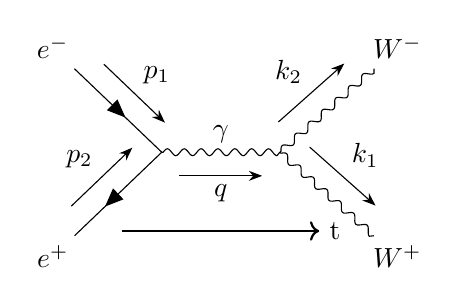
\begin{tikzpicture}[scale=0.5]
        \begin{feynman}
            \vertex (b);
            \vertex [above left=1.5cm of b] (a) {\(e^{-}\)};
            \vertex [below left=1.5cm of b] (e) {\(e^{+}\)};
            \vertex [right=1.5cm of b] (f); 
            \vertex [above right=1.5cm of f] (c) {\(W^{-}\)};
            \vertex [below right=1.5cm of f] (d) {\(W^{+}\)};
            
            \diagram* {
                (a) -- [fermion,momentum={\(p_1\)}] (b),
                (e) -- [anti fermion,momentum={\(p_2\)}] (b),
                (b) -- [boson,momentum'={\(q\)},edge label={\(\gamma\)}] (f),
                (f) -- [boson,momentum={\(k_1\)}] (d),
                (f) -- [boson,momentum={\(k_2\)}] (c)
            };
        \end{feynman}
        \draw[->, thick] (-1,-2) -- (4,-2) node[right] {t};
    \end{tikzpicture}
\end{center}


然后,我们给出其顶点因子以及传播子等:
\subsubsection{光子传播子}
\begin{minipage}{0.5\textwidth}
    \begin{center}
        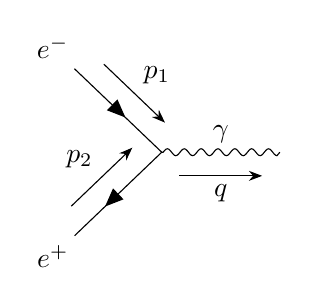
\begin{tikzpicture}[scale=0.5]
            \begin{feynman}
                \vertex (b);
                \vertex [above left=1.5cm of b] (a) {\(e^{-}\)};
                \vertex [below left=1.5cm of b] (e) {\(e^{+}\)};
                \vertex [right=1.5cm of b] (f); 
                
                \diagram* {
                    (a) -- [fermion,momentum={\(p_1\)}] (b),
                    (e) -- [anti fermion,momentum={\(p_2\)}] (b),
                    (b) -- [boson,momentum'={\(q\)},edge label={\(\gamma\)}] (f)
                };
            \end{feynman}
        \end{tikzpicture}
    \end{center}
\end{minipage}
\hfill
\begin{minipage}{0.5\textwidth}
    \begin{equation}
        = \frac{-ig^{\mu\nu}}{q^2}
    \end{equation}
\end{minipage}


其中$q = p_1 + p_2$,此为系统的总动量
\subsubsection{电子光子顶点因子}
这是标准 $QED$ 顶点,其为$-ie\gamma^{\mu}$,我们的正电子旋量为 $\tilde{v}(p_2)$,电子旋量为 $u(p_1)$,因此我们有:
\begin{equation}
    = \tilde{v}(p_2)-ie\gamma^{\mu}u(p_1)
\end{equation}

\subsubsection{$\gamma W^{+}W^{-}$顶点因子}

\begin{minipage}{0.3\textwidth}
    \begin{center}
        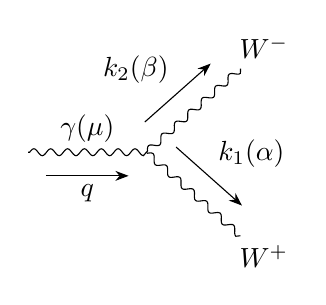
\begin{tikzpicture}[scale=0.5]
            \begin{feynman}
                \vertex (b);
                \vertex [right=1.5cm of b] (f); 
                \vertex [above right=1.5cm of f] (c) {\(W^{-}\)};
                \vertex [below right=1.5cm of f] (d) {\(W^{+}\)};
                
                \diagram* {
                    (b) -- [boson,momentum'={\(q\)},edge label={\(\gamma(\mu)\)}] (f),
                    (f) -- [boson,momentum={\(k_1(\alpha)\)}] (d),
                    (f) -- [boson,momentum={\(k_2(\beta)\)}] (c)
                };
            \end{feynman}
        \end{tikzpicture}
    \end{center}
\end{minipage}
\hfill
\begin{minipage}{0.7\textwidth}
    \begin{equation}
        V_{\alpha\beta\mu} = ie\left[i(k_1 - k_2)_{\mu}g_{\alpha\beta} + i\left(q - k_2\right)_{\alpha}g_{\beta\mu} + i\left(k_2 - q\right)_{\beta}g_{\mu\alpha}\right] 
    \end{equation}
\end{minipage}



由于 $QED$ 当中的电子光子顶点因子太过于常见,我们没有给出其来源,但是 $\gamma W^{+}W^{-}$顶点因子对我而言并不是一个很 trival 的东西,因此我还是给出一部分原因。


给出 $SU(2)_{L} \times U(1)_Y$ 的规范动能项:
\begin{equation}
    \mathcal{L}_{gauge} = -\frac{1}{4}W_{\mu\nu}^{a}W^{a\mu\nu} - \frac{1}{4}B_{\mu\nu}B^{\mu\nu}
\end{equation}

其中
\begin{enumerate}
    \item $\textcolor{blue}{W_{\mu\nu}^{a} = \partial_mu W_{\nu}^a - \partial_\nu W_{\mu}^a} + \textcolor{red}{g \epsilon^{abc}W_\mu^b W_nu^c}$,此为 $SU(2)$的规范场强,蓝色的部分为 $W^+ W^-$ 的动能项,红色部分为非阿贝尔项,也导致了三规范玻色子耦合;
    \item $B_{\mu\nu} = \partial_\mu B_\nu - \partial_\nu B_\mu$,此为 $U(1)$的规范场强; 
\end{enumerate}

这两项便是所有的电弱玻色子的相互作用来源,这时候我们再引入玻色子
\begin{enumerate}
    \item $W_\mu^{\pm} = \frac{1}{\sqrt{2}}(W_\mu^1 \mp i W_\mu^2)$
    \item $Z_\mu = \cos\theta_W W_\mu^3 - \sin\theta_WB_\mu$
    \item $A_\mu = \sin\theta_W W_\mu^3 + \cos\theta_W B_\mu$
\end{enumerate}
电磁相互作用耦合常数(电荷)为: $e = g \sin\theta_W$

此时,我们需要计算的是 $\gamma W^+ W^-$ 的顶点因子,需要注意到的是我们的三玻色子顶点来源于
\begin{equation}
    g\epsilon^{abc}W_\mu^b W_\nu^c
\end{equation}

接着代入 $A$ 与 $W^{\pm}$,首先是计算出平方项
\begin{equation*}
    W_{\mu\nu}^\alpha W^{\alpha\mu\nu} = \left(\partial_\mu W_\nu^\alpha\right)^2 + 2g \epsilon^{abc}\left(\partial_\mu W_\nu^\alpha\right) W^{b\mu}W^{c\nu} + g^2 \left(\epsilon^{abc}W_\mu^b W_\nu^c\right)^2
\end{equation*}

事实上,我们这里计算的是 $\gamma W^+ W^-$ 的三顶点因子,因此我们只取三线性项,即($\partial WWW$)。于是,我们将会取 $SU(2)_L \times U(1)_Y$ 的规范拉格朗日项的三线性项
\begin{align*}
    \mathcal{L}_{3-gauge} &= -\frac{1}{4} \cdot 2g\epsilon^{abc}\left(\partial_\mu W_\nu^\alpha\right) W^{b\mu}W^{c\nu} \\
    &=-\frac{g}{2} \epsilon^{abc} \left(\partial_\mu W_\nu^\alpha\right) W^{b\mu}W^{c\nu} \\
    &= -g \sin \theta_W \left[\left(\partial_\mu W_\nu^+ - \partial_\nu W_\mu^+\right)W^{-\mu}A^\nu + \left(\partial_\mu W_\nu^- - \partial_\nu W_\mu^-\right)W^{+\mu}A^\nu\right] 
\end{align*}

而为了满足规范不变性,还需要加上 $W^+ W^- \partial A$ 项,即
\begin{equation}
    \mathcal{L}_{\gamma WW} = -g \sin \theta_W \left[\left(\partial_\mu W_\nu^+ - \partial_\nu W_\mu^+\right)W^{-\mu}A^\nu + \left(\partial_\mu W_\nu^- - \partial_\nu W_\mu^-\right)W^{+\mu}A^\nu + W_\mu^+ W_\nu^- \left(\partial^\mu A^{\nu} - \partial^\nu A^\mu\right)\right]
\end{equation}

对于此拉格朗日量的规范对称性也容易验证,只需 $A_\mu \to A_\mu + \partial_\mu \alpha$ 代入即可,最终可以得到
\begin{equation*}
    \delta \mathcal{L}_{\gamma WW} = -e\left[W_\mu^+W_\nu^-\left(\partial^\mu\partial^\nu\alpha - \partial^\nu \partial^\mu \alpha\right)\right] = 0
\end{equation*}

很显然我们的三玻色子顶点是满足规范不变性的

\subsubsection{极化玻色子矢量}






\section{计算散射截面}
在计算之前,先定义几个常用的量
\begin{enumerate}
    \item $s = \left(p_1 + p_2\right)^2 = \left(k_1 + k_2\right)^2$
    \item $t = \left(p_1 - k_1\right)^2 = \left(p_2 - k_2\right)^2$
    \item $u = \left(p_1 - k_2\right)^2 = \left(p_2 - k_1\right)^2$
\end{enumerate}

在我们的这个过程当中,存在有这样的关系
\begin{eqnarray*}
    p_1^2 &=& p_2^2 = m_e^2 \\
    k_1^2 &=& k_2^2 = m_W^2 \\
    p_1 \cdot p_2 &=& \frac{s - 2m_e^2}{2} \\
    k_1 \cdot k_2 &=& \frac{s - 2m_W^2}{2} \\
    \left(k_1 - k_2\right)^2 &=& 4m_W^2 - s  \\
\end{eqnarray*}



接下来我们给出三个过程的散射矩阵元,首先给出费曼图:
\begin{center}
    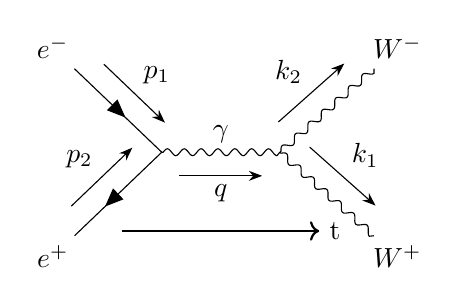
\begin{tikzpicture}[scale=0.5]
        \begin{feynman}
            \vertex (b);
            \vertex [above left=1.5cm of b] (a) {\(e^{-}\)};
            \vertex [below left=1.5cm of b] (e) {\(e^{+}\)};
            \vertex [right=1.5cm of b] (f); 
            \vertex [above right=1.5cm of f] (c) {\(W^{-}\)};
            \vertex [below right=1.5cm of f] (d) {\(W^{+}\)};
            
            \diagram* {
                (a) -- [fermion,momentum={\(p_1\)}] (b),
                (e) -- [anti fermion,momentum={\(p_2\)}] (b),
                (b) -- [boson,momentum'={\(q\)},edge label={\(\gamma\)}] (f),
                (f) -- [boson,momentum={\(k_1\)}] (d),
                (f) -- [boson,momentum={\(k_2\)}] (c)
            };
        \end{feynman}
        \draw[->, thick] (-1,-2) -- (4,-2) node[right] {t};
    \end{tikzpicture}
\end{center}
\begin{eqnarray}
    M_\gamma &=& \bar{v}(p_1)(ie\gamma^\mu)\frac{-ig_{\mu\nu}}{q^2}(-ie)\left[g^{\nu\alpha}(q - k_1)^\beta + g^{\alpha\beta}(k_1 - k_2)^\nu + g^{\beta\nu}(k_2 - q)^\alpha\right]\left(\epsilon_{1\alpha}^* \epsilon_{2\beta}^*\right) \nonumber \\
    &=& -\frac{ie^2}{q^2}\left[\bar{v}(p_1)\gamma^\mu u(p_2)\right]g_{\mu\nu}\left[g^{\nu\alpha}(q - k_1)^\beta + g^{\alpha\beta}(k_1 - k_2)^\nu + g^{\beta\nu}(k_2 - q)^\alpha\right]\left[g_{\alpha\beta} - \frac{k_{1\alpha}k_{2\beta}}{m_W^2}\right] \nonumber \\
    &=& -\frac{ie^2}{q^2} \mathcal{J}_{\gamma}^{\mu}g_{\mu\nu}V^{\nu\alpha\beta}\epsilon_{1\alpha}^* \epsilon_{2\beta}^* \nonumber \\
    M_Z &=& \left[\bar{v}(p_1)\left(-i\frac{g_w}{2\cos{\theta_W}} \gamma^\mu \left(g_V^e - g_A^e \gamma^5\right) u(p_2)\right)\right]\frac{-ig_{\mu\nu}}{q^2 - m_Z^2}(-ig_w \cos{\theta_W})\left[g^{\nu\alpha}(q - k_1)^\beta \right. \nonumber \\
    && \left.+ g^{\alpha\beta}(k_1 - k_2)^\nu + g^{\beta\nu}(k_2 - q)^\alpha\right]\left(\epsilon_{1\alpha}^* \epsilon_{2\beta}^*\right) \nonumber \\
    &=& -\frac{i g_w^2}{2\left(s - m_Z^2\right)}\left[\bar{v}(p_1)\gamma^\mu \left(g_V^e - g_A^e \gamma^5\right) u(p_2)\right]g_{\mu\nu} \left[g^{\nu\alpha}(q - k_1)^\beta + g^{\alpha\beta}(k_1 - k_2)^\nu \right. \nonumber \\
    && \left.+ g^{\beta\nu}(k_2 - q)^\alpha\right]\left(\epsilon_{1\alpha}^* \epsilon_{2\beta}^*\right) \nonumber \\
    &=& -\frac{i g_w^2}{2\left(s - m_Z^2\right)}\mathcal{J}_{Z}^{\mu}g_{\mu\nu}V^{\nu\alpha\beta}\epsilon_{1\alpha}^* \epsilon_{2\beta}^* \nonumber \\
    M_\nu &=& \nonumber
\end{eqnarray}

非常方便的是,我们可以将后面 $V^{\nu\alpha\beta}\epsilon_{1\alpha}^* \epsilon_{2\beta}^*$ 的部分可以进一步化简,变成更为简便的表达
\begin{eqnarray*}
    V^{\nu\alpha\beta}\epsilon_{1\alpha}^* \epsilon_{2\beta}^* &=& \left[g^{\nu\alpha}(q - k_1)^\beta + g^{\alpha\beta}(k_1 - k_2)^\nu + g^{\beta\nu}(k_2 - q)^\alpha\right]\left[g_{\alpha\beta} - \frac{k_{1\alpha}k_{2\beta}}{m_W^2}\right] \\
    &=& \left[g^{\nu\alpha}k_2^\beta + g^{\alpha\beta}(k_1 - k_2)^\nu - g^{\beta\nu}k_1^\alpha\right]\left[g_{\alpha\beta} - \frac{k_{1\alpha}k_{2\beta}}{m_W^2}\right] \\
    &=& \left[k_2^\nu + 4(k_1 - k_2)^\nu - k_1^\nu\right] - \frac{1}{m_W^2}\left[k_2^2 k_1^\nu + (k_1 \cdot k_2) (k_1 - k_2)^\nu - k_1^2 k_2^\nu\right] \\
    &=& \left(3 - \frac{s}{2m_W^2}\right) (k_1 - k_2)^\nu
\end{eqnarray*}




\subsection{计算 $\sigma_{\gamma\gamma}$}
首先我们需要计算 $\left|M_{\gamma}\right|^2$

\begin{eqnarray*}
    \left|M_{\gamma}\right|^2 &=& \frac{g_e^4}{s^2}\left[\bar{v}(p_1)\gamma^\mu u(p_2)\right]\left[\bar{u}(p_2)\gamma^\nu v(p_1)\right]\left(3 - \frac{s}{2m_W^2}\right) (k_1 - k_2)_\mu\left(3 - \frac{s}{2m_W^2}\right) (k_1 - k_2)_\nu
\end{eqnarray*}

接下来我们分别计算前面一部分和后面一部分,首先是前半部分
\begin{eqnarray*}
    \mathbf{Tr}\left[\bar{v}(p_1)\gamma^\mu u(p_2)\right]\left[\bar{u}(p_2)\gamma^\nu v(p_1)\right] &=& \frac{1}{4}\mathbf{Tr} \left[\left(\slashed{p_1} - m_e\right)\gamma^\mu \left(\slashed{p_2} + m_e\right)\gamma^\nu\right] \\
    &=& \frac{1}{4}\Tr\left[\left(\gamma^\sigma p_{1\sigma} - m_e\right)\gamma^\mu \left(\gamma^\rho p_{2\rho} + m_e\right)\gamma^\nu\right] \\
    &=& \frac{1}{4}\Tr\left[\gamma^\sigma \gamma^\mu \gamma^\rho \gamma^\nu p_{1\sigma}p_{2\rho} + \gamma^\sigma \gamma^\mu \gamma^\nu m_e p_{1\sigma} - \gamma^\mu \gamma^\rho \gamma^\nu m_e p_{2\rho} + \gamma^\mu \gamma^\nu m_e^2\right] \\
    &=& \left(g^{\sigma\mu}g^{\rho\nu} - g^{\sigma\rho}g^{\mu\nu} + g^{\sigma\nu}g^{\mu\rho}\right)p_{1\sigma}p_{2\rho} + 0 + 0 + m_e^2g^{\mu\nu} \\
    &=& p_1^\mu p_2^\nu + p_2^\mu p_1^\nu - \left(p_1 \cdot p_2 - m_e^2\right)g^{\mu\nu}
\end{eqnarray*}

接下来将我们前面得到的极化求和部分和电子流的部分结合起来,就可以得到完整的散射振幅


\begin{eqnarray*}
    \left|M_\gamma\right|^2 &=& \frac{g_e^4}{s^2}\left[p_1^\mu p_2^\nu + p_2^\mu p_1^\nu - \left(p_1 \cdot p_2 - m_e^2\right)g^{\mu\nu}\right] \left(3 - \frac{s}{2m_W^2}\right)^2 (k_1 - k_2)_\nu (k_1 - k_2)_\mu \\
    &=& \frac{g_e^4}{s^2} \left(3 - \frac{s}{2m_W^2}\right)^2 \left[2 \ p_1 \cdot (k_1 - k_2) p_2 \cdot (k_1 - k_2) - \left(p_1 \cdot p_2 - m_e^2\right)\left(k_1 - k_2\right)^2\right] \\
    &=& \frac{g_e^4}{s^2} (-\frac{1}{2})\left(3 - \frac{s}{2m_W^2}\right)^2\left[(u - t)^2 + \left(s - 4m_e^2 \right)\left(s - 4m_W^2\right)\right] \\
    &=& -\frac{g_e^4}{2s^2}\left(3 - \frac{s}{2m_W^2}\right)^2\left[(u - t)^2 + \left(s - 4m_e^2 \right)\left(s - 4m_W^2\right)\right] \\
    &=& -\frac{g_e^4}{2s^2}\left(3 - \frac{s}{2m_W^2}\right)^2 \left(s - 4m_e^2 \right)\left(s - 4m_W^2\right) \left(1 + \cos^2{\theta}\right)
\end{eqnarray*}


另外我们的散射截面与散射矩阵元的关系有
\begin{eqnarray*}
    \sigma_{\gamma\gamma} &=& \int \frac{d\sigma}{d\Omega} d\Omega \\
    &=& \int \frac{d\sigma}{d\Omega} sin\theta d\phi d\theta \\
    &=& -\int_{0}^{2\pi} d\phi \int_{-1}^{1} \frac{d\sigma}{d\Omega} d(\cos{\theta}) \\
    &=& -\frac{1}{32 \pi s} \int_{-1}^{1} \frac{|p_f|}{|p_i|} \left|M_\gamma\right|^2 d(\cos{\theta})
\end{eqnarray*}

同时
\begin{eqnarray*}
    \frac{|p_f|}{|p_i|} &=& \sqrt{\frac{s - 4m_W^2}{s - 4m_e^2}} \\
    g_e &=& \sqrt{4\pi\alpha}
\end{eqnarray*}

通过简单的积分计算,我们得到了
\begin{equation}
    \sigma_{\gamma\gamma} = \frac{2 \pi \alpha^2}{3s^3}\left(3 - \frac{s}{2m_W^2}\right)^2 \left(s - 4m_e^2 \right)^{\frac{1}{2}}\left(s - 4m_W^2\right)^{\frac{3}{2}}
\end{equation}

\subsection{计算 $\sigma_{ZZ}$}






\section{计算结果以及可视化}

经过我们的计算,我们最终可以将结果总结为\cite{commins1985weak}
\begin{align*}
    \bar{\sigma}_{\nu\nu} &= \sigma_1 \\
    \bar{\sigma}_{\gamma\gamma} &= x^2 \sigma_2\\
    \bar{\sigma}_{ZZ} &= \left(x^2 - \frac{1}{2}x + \frac{1}{8}\right)\frac{s^2}{\left(s - m_z^2\right)^2}\sigma_2\\
    \bar{\sigma}_{Z\gamma} &= 2\left(\frac{1}{4} - x\right)\frac{s}{\left(s - m_z^2\right)}\sigma_2\\
    \bar{\sigma}_{\nu Z} &= \left(x - \frac{1}{2}\right)\frac{s}{\left(s - m_z^2\right)}\sigma_3\\
    \bar{\sigma}_{\gamma \nu} &= -x\sigma_3\\
    \sigma_{tot} &= \frac{\pi \alpha^2}{8 x^2} \beta \frac{1}{s} \sum_{ij}\bar{\sigma}_{ij} \\
\end{align*}

其中,
\begin{align*}
    \sigma_1 &= 2 \frac{s}{m_W^2} + \frac{1}{12} \left(\frac{s}{m_W^2}\right)^2 \beta^2 + 4\left(\frac{1 - 2 m_W^2}{s}\frac{L}{\beta} - 1\right) \\
    \sigma_2 &= 16 \frac{s}{m_W^2}\beta^2 + \frac{2}{3} \beta^2 \left[\left(\frac{s}{m_W^2}^2 - 4\frac{s}{m_W^2} + 12\right)\right] \\
    \sigma_3 &= 16 - 32 \frac{m_W^2}{s} \frac{L}{\beta} + 8\beta^2 \frac{s}{m_W^2} + \frac{1}{3} \beta^2\left(\frac{s}{m_W^2}\right)^2 \left(1 - 2\frac{m_W^2}{s}\right) + 4\left(1 - 2\frac{m_W^2}{s}\right) - 16\left(\frac{m_W^2}{s}\right)^2\frac{L}{\beta} \\
\end{align*}

其中,我们的 $\displaystyle \beta = \left(1 - 4 \frac{m_W^2}{s}\right)^{\frac{1}{2}}$ , $\displaystyle x = \sin^2\theta_W$ , $\displaystyle L = \ln\left|\frac{1 + \beta}{1 - \beta}\right|$






\newpage
%%
%\begin{center}
%    \begin{thebibliography}{999}
%        \bibitem{000} arXiv:2501.08354 [hep-ph]
%        \bibitem{001} Eugene D. Commins, Philip H. Bucksbaum,Weak Interactions of Leptons and Quarks.
%    \end{thebibliography}
%\end{center}

\begin{center}
    \bibliographystyle{plain} % 样式
    \bibliography{reference.bib} % yourfile为BibTeX文件名,不需要扩展名
    \nocite{Veltman_1994}
    \nocite{Peskin:1995ev}
    \nocite{Paschos_2023a}
\end{center}




\end{document}
